\documentclass{scrartcl}
\usepackage[top=4cm,left=2.5cm,right=3cm,bottom=5cm]{geometry}
\usepackage[latin1]{inputenc}
\usepackage[ngerman]{babel}
\usepackage{amsmath}
\usepackage{amsfonts}
\usepackage{amssymb}
\usepackage{graphicx}
\usepackage{mathabx} % contains \Dashv
\usepackage{enumitem}
\usepackage{fancyhdr}

\title{Informatik der Syteme - Exercise 3}
\author{Jan Hoffmann}
\pagestyle{fancy}
% Header
\fancyhead[L]{\textbf{Informatik der Systeme}\\ \textbf{Exercise 3}}
\fancyhead[C]{}
\fancyhead[R]{Jan Hoffmann, Matr. 3177642\\ Mike Hengge, Matr. 3940400}
% Footer
\fancyfoot[L]{}
\fancyfoot[C]{}
\fancyfoot[R]{\thepage}

\SetLabelAlign{Top}{#1\vfill}

\begin{document}

\section*{Problem 3.1:}
	\begin{enumerate}
		\item \text{} \\
				\begin{tabular}{l|l|c}
				7 & Application & HTTP \\ \hline
				6 & Presentation & \\ \hline
				5 & Session & \\ \hline
				4 & Transport & TCP \\ \hline 
				3 & Network & IP \\ \hline
				2 & Data Link & Ethernet \\ \cline{1-2}
				1 & Physical & WLAN
			\end{tabular}
		
		\item		
			Das Domain Name System (DNS) l�st eine URL in eine IP-Adresse des Ziel Servers auf.
			
		\item 
			Die HTTP-Daten werden zu erst auf der Anwendungsschicht mit einem TCP-Header versehen, 
			dann auf der Netzwerkschicht mit einem IP-Header in dem die IP-Adresse des Zielservers steht (aus dem DNS Protokoll). 
			Dann wird das Ganze in der Vermittlungsschicht mit einem Ethernet-Header versehen, in dem das Interface des Routers
			definiert wird. Dann wird das Packet �ber WLAN and den Router gesendet. Der Router schaut sich die IP-Adresse an und
			versendet an die MAC-Adresse des Zielservers ins Internet. Dort wird das Packet (�ber ein Switch, das ins Internet die 
			MAC des Zielservers repr�sentiert) zum Zielserver gerouted. Der packt Schicht um Schicht mit den jeweiligen Protokollen 
			in den jeweiligen Layern wieder aus.
			
			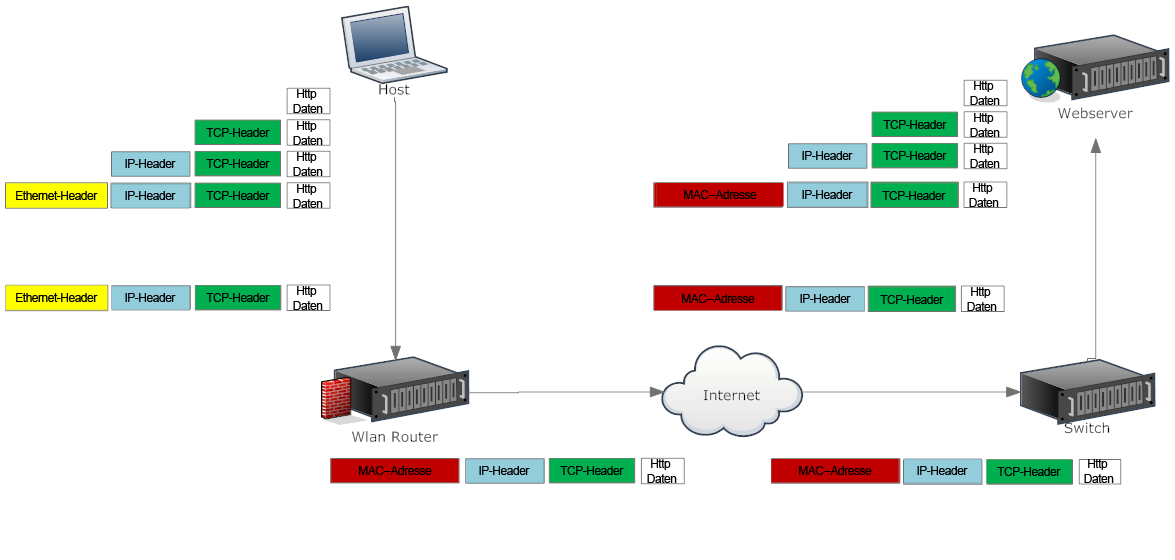
\includegraphics[width=\linewidth]{3_1_3.png}
			
	\end{enumerate}
	
		
\newpage		
\section*{Problem3.2:}
		\begin{enumerate}
			\item % 1.
				$\setlength{\arraycolsep}{0pt}
				\begin{array}[t]{*{16}{l}}
					1&0&0&0&0&0&0&0&0&0&0&0&0&0&0&1\\
					1&1&0&0&1& & & & & & & & & & & \\ \cline{1-5}
					 &1&0&0&1&0& & & & & & & & & & \\
					 &1&1&0&0&1& & & & & & & & & & \\\cline{2-6}
					 & &1&0&1&1&0& & & & & & & & & \\
					 & &1&1&0&0&1& & & & & & & & & \\\cline{3-7}
					 & & &1&1&1&1&0& & & & & & & & \\
					 & & &1&1&0&0&1& & & & & & & & \\\cline{4-8}
					 & & & & &1&1&1&0&0& & & & & & \\
					 & & & & &1&1&0&0&1& & & & & & \\\cline{6-10}
					 & & & & & & &1&0&1&0&0& & & & \\
					 & & & & & & &1&1&0&0&1& & & & \\\cline{8-12}
					 & & & & & & & &1&1&0&1&0& & & \\
					 & & & & & & & &1&1&0&0&1& & & \\\cline{9-13}
					 & & & & & & & & & & &1&1&0&0&1\\
					 & & & & & & & & & & &1&1&0&0&1\\\cline{12-16}
					 & & & & & & & & & & & & & & &0\\
				\end{array}:11001=11110101001 \Rightarrow primitiv$
				
				$\setlength{\arraycolsep}{0pt}
				\begin{array}[t]{*{16}{l}}
					1&0&0&0&0&0&0&0&0&0&0&0&0&0&0&1\\
					1&0&1&1&1& & & & & & & & & & & \\ \cline{1-5}
					 &0&1&1&1&0&0& & & & & & & & & \\
					 & &1&0&1&1&1& & & & & & & & & \\ \cline{3-7}
					 & & &1&0&1&1&0& & & & & & & & \\
					 & & &1&0&1&1&1& & & & & & & & \\ \cline{4-8}
					 & & & & & & &1&0&0&0&0& & & & \\
					 & & & & & & &1&0&1&1&1& & & & \\ \cline{8-12}
					 & & & & & & & &0&1&1&1&0&0& & \\
					 & & & & & & & & &1&0&1&1&1& & \\ \cline{10-14}
					 & & & & & & & & & &1&0&1&1&0& \\
					 & & & & & & & & & &1&0&1&1&1& \\ \cline{11-15}
					 & & & & & & & & & &0&0&0&1&1& \\							
				\end{array}:10111=101100010110 \ Rest \ 11 \Rightarrow \ nicht \ primitiv$
				
				$\setlength{\arraycolsep}{0pt}
				\begin{array}[t]{*{16}{l}}
					1&0&0&0&0&0&0&0&0&0&0&0&0&0&0&1\\
					1&1&0&1&1& & & & & & & & & & & \\ \cline{1-5}
					 &1&0&1&1&0& & & & & & & & & & \\
					 &1&1&0&1&1& & & & & & & & & & \\ \cline{2-6}
					 & &1&1&0&1&0& & & & & & & & & \\
					 & &1&1&0&1&1& & & & & & & & & \\ \cline{3-7}
					 & & & & & &1&0&0&0&0& & & & & \\
					 & & & & & &1&1&0&1&1& & & & & \\ \cline{7-11}
					 & & & & & & &1&0&1&1&0& & & & \\
					 & & & & & & &1&1&0&1&1& & & & \\ \cline{8-12}
					 & & & & & & & &1&1&0&1&0& & & \\
					 & & & & & & & &1&1&0&1&1& & & \\ \cline{9-13}
					 & & & & & & & & &0&0&0&1&0&0&1 \\
				\end{array}:10111=111000111000 \ Rest \ 1001 \Rightarrow \ nicht \ primitiv$
							
			\item % 2.
				$\setlength{\arraycolsep}{0pt}
				\begin{array}[t]{*{5}{l}}
					1&1&0&0&1\\
					1&1& & & \\ \cline{1-2}
					 & &0&0&1\\								
				\end{array}:11=1000 \ Rest \ 1 \Rightarrow \ nicht \ durch \ 11 \ teilbar. $
				
				$\setlength{\arraycolsep}{0pt}
				\begin{array}[t]{*{6}{l}}
					1&0&1&1&1& \\
					1&1& & & & \\ \cline{1-2}
					 & &1&1& & \\
					 & &1&1& & \\ \cline{3-4}
					 & & &0&1&1\\
					 & & & &1&1\\ \cline{5-6}
					 & & & &0&0								
				\end{array}:11=1000 \ Rest \ 0 \Rightarrow \ durch \ 11 \ teilbar. $
				
				$\setlength{\arraycolsep}{0pt}
				\begin{array}[t]{*{5}{l}}
					1&1&0&1&1\\
					1&1\\ \cline{1-2}
					 &0&0&1&1\\
					 & & &1&1\\ \cline{4-5}
					 & & &0&0\\
				\end{array}:11=1001 \ Rest \ 0 \Rightarrow \ durch \ 11 \ teilbar.$
			
			\item
				Durch die alternierende Quersumme des Polynoms kann man einfach sehen, ob es durch u + 1 teilbar ist. \\
				Dazu muss nur abwechselnd jede Stelle des Polynoms zu der vorigen addiert bzw. davon abgezogen werden. 
				Ist die verbleibende Zahl durch 3 teilbar, so ist es auch das Ursprungspolynom. \\
				Beispiel: $1001 \Rightarrow 1 + 0 - 0 + 1 = 11 \Rightarrow$ durch \  11 \ teilbar. 		
				
		\end{enumerate}

\newpage
\section*{Problem3.3:}
	\begin{enumerate}
		\item % 1.
			\begin{align*}	% aligns equations on '=' with '&='		
				%\label{eq:} % label is usefull for \ref{label} 
				H^* &= \sum\nolimits_{1<i\leq N} p(x_i) * ld (\frac{1}{p(x_i)}) bit \\
				H^* &= p(x_1) * ld (\frac{1}{p(x_1))} 
						 + p(x_2) * ld (\frac{1}{p(x_2)}) 
						 + p(x_3) * ld (\frac{1}{p(x_3)}) 
						 + p(x_4) * ld (\frac{1}{p(x_4)})  \\
						&\qquad + p(x_5) * ld (\frac{1}{p(x_5)}) 
						 +p (x_6) * ld (\frac{1}{p(x_6)}) 
						 + p(x_7) * ld (\frac{1}{p(x_7)} bit \\
						&= 0,10 * ld (10) + 0,30 * ld (\frac{10}{3}) + 0,10 * ld (10) + 0,10 * ld (10) + 0,15 * ld (\frac{20}{3}) \\
						&\qquad + 0,10 * ld (10) + 0,15 * ld (\frac{20}{3}) bit \\
						&= 0,30 * ld (\frac{10}{3}) + 2 * 0,15 * ld (\frac{20}{3}) + 4 * 0,10 * ld(10) bit \\
						&\approx 1,3288 + 0,8210898 + 0,5210896   bits \\
						&\approx 2,67 bits 			
			\end{align*}
		
		\item % 2.
			\text{} \\
			\begin{figure}[h]%
				\begin{center}
					\begin{minipage}[t]{0.4\linewidth}
						\begin{tabular}[b]{|l|l|} 	% | macht die vertikalen striche; l r c erzeugt je eine Spalte mit entsprechnder B�ndigkeit
							\hline 										% erste horizontale Linie (�ber der Tabelle)
							Zeichen & Optimalcodierung \\ \hline
							$x_2$   & 0                \\ \hline
							$x_5$   & 100              \\ \hline
							$x_7$   & 101              \\ \hline
							$x_1$   & 1100             \\ \hline 
							$x_3$   & 1101             \\ \hline
							$x_4$   & 1110             \\ \hline
							$x_6$   & 1111	           \\ \hline			
						\end{tabular}
					\end{minipage}
					\hspace{0.1\linewidth}
					\begin{minipage}[t]{0.4\linewidth}				
						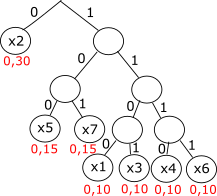
\includegraphics[scale=0.75]{algorithm.png}
					\end{minipage}	
					%\caption{}%
					%\label{}%
				\end{center}
			\end{figure}
			
		\item % 3.
			\begin{align*}
				R_c &= S_m - H^* \\
				S_m &=  \sum\nolimits_{1<i\leq N} S_i * p(x_i) bit \\
				&= 1 * 0,30 + 2 * 3 * 0,15 + 4 * 4 * 0,10 bit\\
				&= 2,8 bit\\
				\Rightarrow R_c &= 2,8 - 2,67 = 0,13
			\end{align*}		
			Bei einer Codierung mit einheitlichen Bin�rstellenzahl werden 3 bit ben�tigt,
			um alle sieben verschiedenen Zeichen darzustellen.\\
			\begin{align*}
				\Rightarrow S_m &= 3 * 0,30 + 2 * 3 * 0,15 + 4 * 3 * 0,10 bit \\
				&= 3 bit \\
				\Rightarrow R_c &= 3 - 2,67 = 0,33 
			\end{align*}
			Die Optimalcodierung hat sogar bei nur sieben Zeichen bereits eine deutlich niedrigere Coderedundanz. 
			
	\end{enumerate}
\end{document}